\section{Transfer Learning}

Transfer learning is when a model is train for one task and try to use that knowledge for another related task, usually within the same domain.  Figure \ref{fig:transfer} shows some intuitive examples inspired by human ability to relatively easily transfer the knowledge learned from the task on the wright of the arrows to the ones on the left. This idea have been applied to ML across all domains. In this project, we leveraged this idea by transferring the knowledge from a model that was trained on ImageNet dataset for the problem of shoes classification.

Xception \cite{chollet2017xception} was proposed in 2017 by Chollet. It is a convolutional neural network that is 126 layers deep and it was pretrained on the ImageNet dataset. The architect of this model take inspiration form Inception, but the Inception modules were replaced with depthwise separable convolutions. In-spite of the depth, this this make more efficient use of the model parameters, which even lead to better performance. Also, it is ranked the top 1 accuracy on kearas applications. Thus, it is a good fit to our problem. 

\begin{figure}[h]
  \centering
  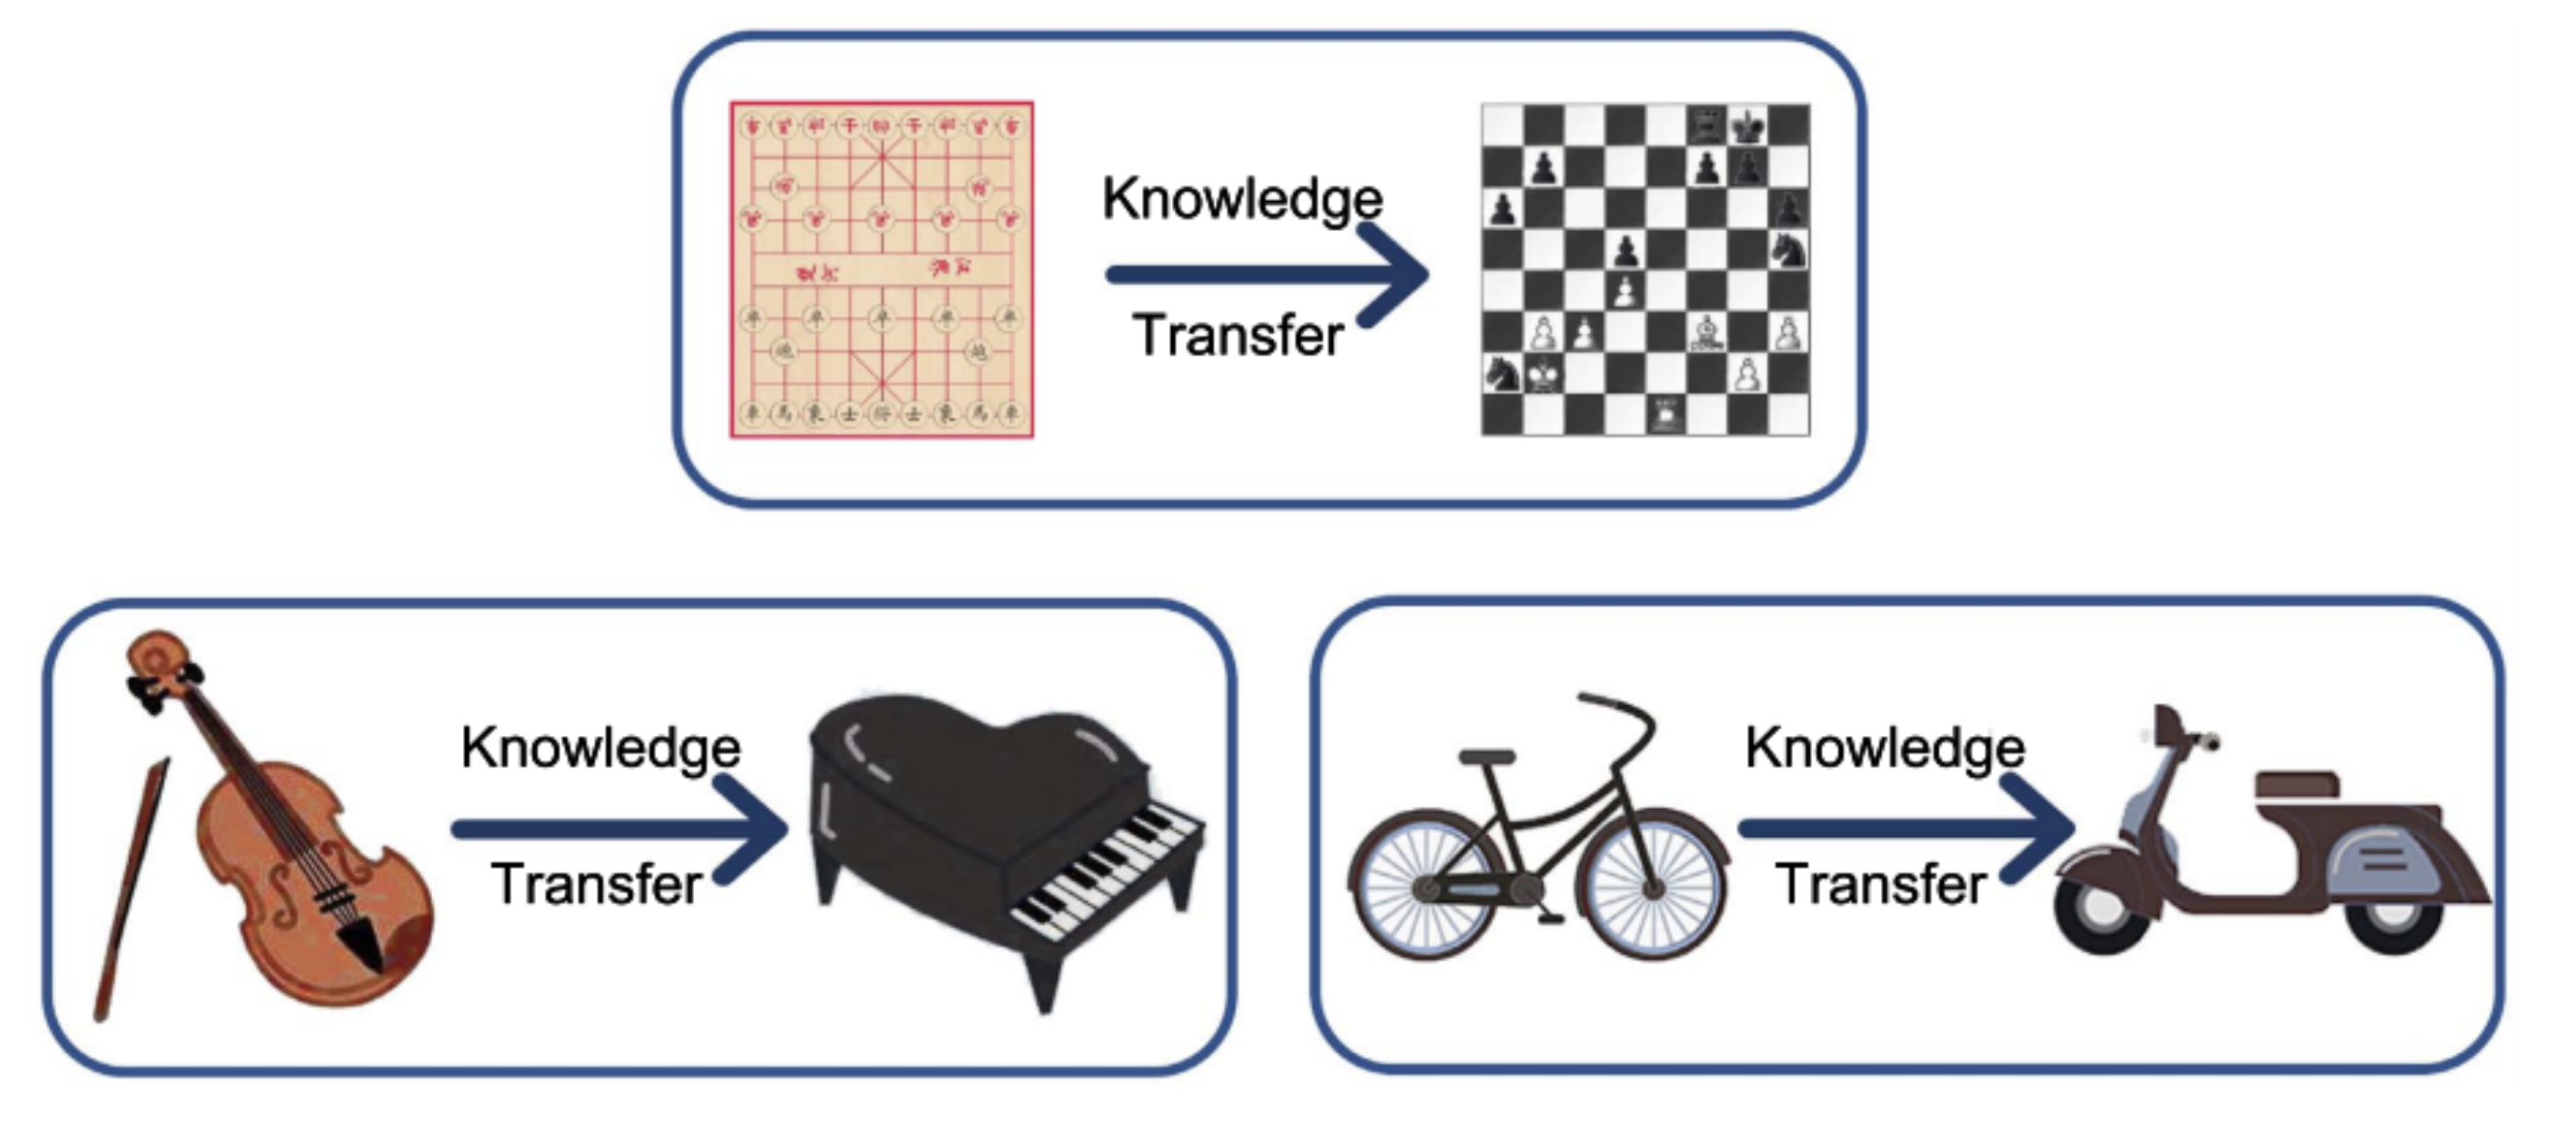
\includegraphics[width=\linewidth]{figs/transfer_learning.png}
  \caption{Intuitive examples about transfer learning.}
  \label{fig:transfer}
\end{figure}